\documentclass[book,11pt]{IEEEtran}
\usepackage{setspace}
\usepackage{gensymb}
\singlespacing
\usepackage[cmex10]{amsmath}
\usepackage{amsthm}
\usepackage{mathrsfs}
\usepackage{txfonts}
\usepackage{stfloats}
\usepackage{bm}
\usepackage{cite}
\usepackage{cases}
\usepackage{subfig}
\usepackage{longtable}
\usepackage{multirow}
\usepackage{enumitem}
\usepackage{mathtools}
\usepackage{tikz}
\usepackage{circuitikz}
\usepackage{verbatim}
\usepackage[breaklinks=true]{hyperref}
\usepackage{tkz-euclide} % loads  TikZ and tkz-base
\usepackage{listings}
\usepackage{color}    
\usepackage{array}    
\usepackage{longtable}
\usepackage{calc}     
\usepackage{multirow} 
\usepackage{hhline}   
\usepackage{ifthen}   
\usepackage{lscape}     
\usepackage{chngcntr}
\usepackage{float}
\DeclareMathOperator*{\Res}{Res}
\renewcommand\thesection{\arabic{section}}
\renewcommand\thesubsection{\thesection.\arabic{subsection}}
\renewcommand\thesubsubsection{\thesubsection.\arabic{subsubsection}}

\renewcommand\thesectiondis{\arabic{section}}
\renewcommand\thesubsectiondis{\thesectiondis.\arabic{subsection}}
\renewcommand\thesubsubsectiondis{\thesubsectiondis.\arabic{subsubsection}}
\renewcommand\thetable{\arabic{table}}
% correct bad hyphenation here
\hyphenation{op-tical net-works semi-conduc-tor}
\def\inputGnumericTable{}                                 %%

\lstset{
%language=C,
frame=single, 
breaklines=true,
columns=fullflexible
}
%\lstset{
%language=tex,
%frame=single, 
%breaklines=true
%}

\title{Random vector}
\author{Barath surya M | EE22BTECH11014}
\begin{document}
\newtheorem{theorem}{Theorem}[section]
\newtheorem{problem}{Problem}
\newtheorem{proposition}{Proposition}[section]
\newtheorem{lemma}{Lemma}[section]
\newtheorem{corollary}[theorem]{Corollary}
\newtheorem{example}{Example}[section]
\newtheorem{definition}[problem]{Definition}
\newcommand{\BEQA}{\begin{eqnarray}}
\newcommand{\EEQA}{\end{eqnarray}}
\newcommand{\define}{\stackrel{\triangle}{=}}
\bibliographystyle{IEEEtran}
\providecommand{\mbf}{\mathbf}
\providecommand{\pr}[1]{\ensuremath{\Pr\left(#1\right)}}
\providecommand{\qfunc}[1]{\ensuremath{Q\left(#1\right)}}
\providecommand{\sbrak}[1]{\ensuremath{{}\left[#1\right]}}
\providecommand{\lsbrak}[1]{\ensuremath{{}\left[#1\right.}}
\providecommand{\rsbrak}[1]{\ensuremath{{}\left.#1\right]}}
\providecommand{\brak}[1]{\ensuremath{\left(#1\right)}}
\providecommand{\lbrak}[1]{\ensuremath{\left(#1\right.}}
\providecommand{\rbrak}[1]{\ensuremath{\left.#1\right)}}
\providecommand{\cbrak}[1]{\ensuremath{\left\{#1\right\}}}
\providecommand{\lcbrak}[1]{\ensuremath{\left\{#1\right.}}
\providecommand{\rcbrak}[1]{\ensuremath{\left.#1\right\}}}
\theoremstyle{remark}
\newtheorem{rem}{Remark}
\newcommand{\sgn}{\mathop{\mathrm{sgn}}}
\providecommand{\abs}[1]{\left\vert#1\right\vert}
\providecommand{\res}[1]{\Res\displaylimits_{#1}} 
\providecommand{\norm}[1]{\left\lVert#1\right\rVert}
\providecommand{\mtx}[1]{\mathbf{#1}}
\providecommand{\mean}[1]{E\left[ #1 \right]}
\providecommand{\fourier}{\overset{\mathcal{F}}{ \rightleftharpoons}}
\providecommand{\system}[1]{\overset{\mathcal{#1}}{ \longleftrightarrow}}
\newcommand{\solution}{\noindent \textbf{Solution: }}
\newcommand{\cosec}{\,\text{cosec}\,}
\providecommand{\dec}[2]{\ensuremath{\overset{#1}{\underset{#2}{\gtrless}}}}
\newcommand{\myvec}[1]{\ensuremath{\begin{pmatrix}#1\end{pmatrix}}}
\newcommand{\mydet}[1]{\ensuremath{\begin{vmatrix}#1\end{vmatrix}}}
\let\vec\mathbf
\def\putbox#1#2#3{\makebox[0in][l]{\makebox[#1][l]{}\raisebox{\baselineskip}[0in][0in]{\raisebox{#2}[0in][0in]{#3}}}}
     \def\rightbox#1{\makebox[0in][r]{#1}}
     \def\centbox#1{\makebox[0in]{#1}}
     \def\topbox#1{\raisebox{-\baselineskip}[0in][0in]{#1}}
     \def\midbox#1{\raisebox{-0.5\baselineskip}[0in][0in]{#1}}
\maketitle
\vspace{3cm}
Consider a triangle with vertices
		\begin{align}
			\label{eq:tri-pts}
			\vec{A} = \myvec{-3 \\ -4},\,
			\vec{B} = \myvec{-1 \\ 3},\,
			\vec{C} = \myvec{1 \\ -5}
		\end{align}
\section{Vectors}
\documentclass[journal,12pt,two column]{IEEEtran}
%\usepackage{setspace}
\usepackage{amssymb}
\usepackage[cmex10]{amsmath}
\usepackage{amsthm}
\usepackage[export]{adjustbox}
\usepackage{bm}
\def\inputGnumericTable{} 

\usepackage[latin1]{inputenc}                                 
\usepackage{color}                                            
\usepackage{array} 
\usepackage{longtable} 
\usepackage{calc}                                             
\usepackage{multirow}                                         
\usepackage{hhline}                                           
\usepackage{ifthen}  
\usepackage{mathtools}
\usepackage{tikz}
\usepackage{listings}
\usepackage{color}                                            %%
\usepackage{array}                                            %%
\usepackage{caption} 
\usepackage{graphicx}
\renewcommand\thesection{\arabic{section}}
\renewcommand\thesubsection{\thesection.\arabic{subsection}}
\renewcommand\thesubsubsection{\thesubsection.\arabic{subsubsection}}

\renewcommand\thesectiondis{\arabic{section}}
\renewcommand\thesubsectiondis{\thesectiondis.\arabic{subsection}}
\renewcommand\thesubsubsectiondis{\thesubsectiondis.\arabic{subsubsection}}
\title{Assignment}
\author{Barath surya M \\ EE22BTECH11014}

% correct bad hyphenation here
\hyphenation{op-tical net-works semi-conduc-tor}
\def\inputGnumericTable{}                                 %%

\lstset{
%language=C,
frame=single, 
breaklines=true,
columns=fullflexible
}
%\lstset{
%language=tex,
%frame=single, 
%breaklines=true
%}


\providecommand{\pr}[1]{\ensuremath{\Pr\left(#1\right)}}
\providecommand{\prt}[2]{\ensuremath{p_{#1}^{\left(#2\right)} }}        % own macro for this question
\providecommand{\qfunc}[1]{\ensuremath{Q\left(#1\right)}}
\providecommand{\sbrak}[1]{\ensuremath{{}\left[#1\right]}}
\providecommand{\lsbrak}[1]{\ensuremath{{}\left[#1\right.}}
\providecommand{\rsbrak}[1]{\ensuremath{{}\left.#1\right]}}
\providecommand{\brak}[1]{\ensuremath{\left(#1\right)}}
\providecommand{\lbrak}[1]{\ensuremath{\left(#1\right.}}
\providecommand{\rbrak}[1]{\ensuremath{\left.#1\right)}}
\providecommand{\cbrak}[1]{\ensuremath{\left\{#1\right\}}}
\providecommand{\lcbrak}[1]{\ensuremath{\left\{#1\right.}}
\providecommand{\rcbrak}[1]{\ensuremath{\left.#1\right\}}}
\newcommand{\sgn}{\mathop{\mathrm{sgn}}}
\providecommand{\abs}[1]{\left\vert#1\right\vert}
\providecommand{\res}[1]{\Res\displaylimits_{#1}} 
\providecommand{\norm}[1]{\left\lVert#1\right\rVert}
%\providecommand{\norm}[1]{\lVert#1\rVert}
\providecommand{\mtx}[1]{\mathbf{#1}}
\providecommand{\mean}[1]{E\left[ #1 \right]}
\providecommand{\cond}[2]{#1\middle|#2}
\providecommand{\fourier}{\overset{\mathcal{F}}{ \rightleftharpoons}}
%\providecommand{\hilbert}{\overset{\mathcal{H}}{ \rightleftharpoons}}
%\providecommand{\system}{\overset{\mathcal{H}}{ \longleftrightarrow}}
 %\newcommand{\solution}[2]{\textbf{Solution:}{#1}}
\newcommand{\solution}{\noindent \textbf{Solution: }}
\newcommand{\cosec}{\,\text{cosec}\,}
\providecommand{\dec}[2]{\ensuremath{\overset{#1}{\underset{#2}{\gtrless}}}}
\newcommand{\myvec}[1]{\ensuremath{\begin{pmatrix}#1\end{pmatrix}}}
\newcommand{\mydet}[1]{\ensuremath{\begin{vmatrix}#1\end{vmatrix}}}
\providecommand{\rank}{\text{rank}}
\providecommand{\pr}[1]{\ensuremath{\Pr\left(#1\right)}}
\providecommand{\qfunc}[1]{\ensuremath{Q\left(#1\right)}}
 \newcommand*{\permcomb}[4][0mu]{{{}^{#3}\mkern#1#2_{#4}}}
\newcommand*{\perm}[1][-3mu]{\permcomb[#1]{P}}
\newcommand*{\comb}[1][-1mu]{\permcomb[#1]{C}}
\providecommand{\qfunc}[1]{\ensuremath{Q\left(#1\right)}}
\providecommand{\gauss}[2]{\mathcal{N}\ensuremath{\left(#1,#2\right)}}
\providecommand{\diff}[2]{\ensuremath{\frac{d{#1}}{d{#2}}}}
\providecommand{\myceil}[1]{\left \lceil #1 \right \rceil }
\newcommand\figref{Fig.~\ref}
\newcommand\tabref{Table~\ref}
\newcommand{\sinc}{\,\text{sinc}\,}
\newcommand{\rect}{\,\text{rect}\,}
%%
% %\newcommand{\solution}[2]{\textbf{Solution:}{#1}}
%\newcommand{\solution}{\noindent \textbf{Solution:

%\newcommand{\cosec}{\,\text{cosec}\,}
%\numberwithin{equation}{section}
%\numberwithin{equation}{subsection}
%\numberwithin{problem}{section}
%\numberwithin{definition}{section}
%\makeatletter
%\@addtoreset{figure}{problem}
%\makeatother

%\let\StandardTheFigure\thefigure
\let\vec\mathbf

\begin{document}
\maketitle
Consider the experiment of throwing a die. If a multiple of 3 comes up, throw the die again. If any other number comes up, toss a coin. Find the conditional probability of the event the coin shows a tail, given that  at least one die shows a 3.\\
\solution
Let, the states $S_0$ and $S_1$ describe the outcomes of dice throws.\\
$S_2$ and $S_3$ describe the outcomes of coin toss.
\begin{align}
    S_0 &= \Sigma{\brak{Y=k}} ;k\in{\brak{3,6}}\\
    S_1 &= \Sigma{\brak{Y=k}} ; k\in{\brak{1,2,4,5}}\\
    S_2 &= \text{Outcome of coin toss is heads}\\
    S_3 &= \text{Outcome of coin toss is tails}
\end{align}
Conditional Probability is that "The coin shows tails" given that "at least one die shows a 3".
Since, a Markov chain does not depend on the past outcomes,
\begin{align}
    P_{\brak{S_3 | S_0}}&=P_r\brak{X_n=S_3|X_1 =S_0}
\end{align}
Transition Probability Matrix is given as,
\begin{align}
    P&=\myvec{\frac{1}{3}&\frac{2}{3}&0&0\\
                0&0&\frac{1}{2}&\frac{1}{2}\\
                0&0&1&0\\
                0&0&0&0
                }
\end{align}
And State vector is ,
\begin{align}
    Q_0=\myvec{1&0&0&0}
\end{align}
Since the chain starts form $S_0$ according to Markov chain.
The long term Probability that system will be in each state is called stationary state, and stationary state probability is given as,
\begin{align}
    A\pi&=\pi
\end{align}
where $\pi$ is steady state probability vector.\\So,after long time,
\begin{align}
    Q_1&=Q_0 P\\
    Q_2&=Q_1 P \\
    \vdots\\
    Q_{n}&=Q_{n-1} P
\end{align}
So substituting the state vectors we get,
\begin{align}
    Q_{n}&=Q_0 P^{n}\\
\end{align}
applying limits to find the stationary probability vector,
\begin{align}
     \lim_{n \to \infty} Q_{n}&=Q_0 P^{n}
\end{align} \label{eq:steady}
By substituting the values of $Q_0$ and $P$ in the above equation, We get the steady state probability vector as,
\begin{align}
    \pi&=\myvec{0&0&\frac{1}{2}&\frac{1}{2}}
\end{align}
So, the probability that "coin shows tails" given that "Die shows at least one 3" is,
\begin{align}
    p_{\brak{3|1}} &= \frac{1}{2}
\end{align}
\begin{figure}[ht!]
    \centering
    \resizebox{.9\linewidth}{!}{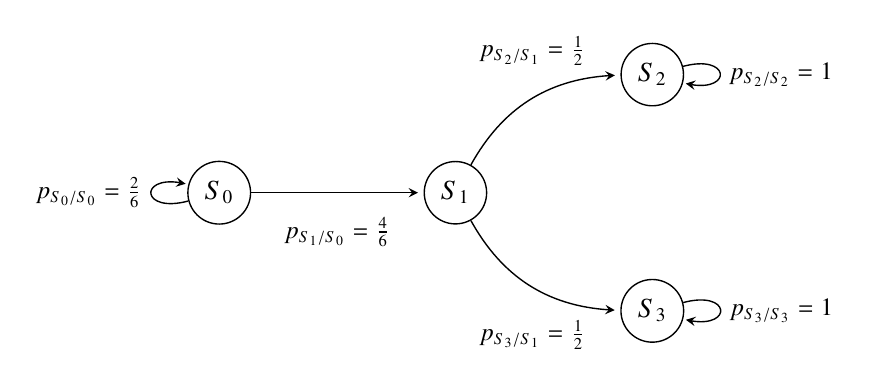
\begin{tikzpicture}[->, >= stealth, shorten >=2pt, line width=0.5pt, node distance=2cm]
  \node[circle, draw] (A) at (0, 1.5) {$S_0$};
  \node[circle, draw] (B) at (3, 1.5) {$S_1$};
  \node[circle, draw] (C) at (5.5, 3) {$S_2$};
  \node[circle, draw] (D) at (5.5, 0) {$S_3$};
  
  \begin{small}
    \path (A) edge [loop left] node [left] {$p_{S_0/S_0} = \frac{2}{6}$} (A);
    \path (A) edge node [below = 0.2cm] {$p_{S_1/S_0} = \frac{4}{6}$} (B);
  
    \path (B) edge [bend left] node [above = 0.3cm] {$p_{S_2/S_1} = \frac{1}{2}$} (C);
    \path (B) edge [bend right] node [below = 0.3cm] {$p_{S_3/S_1} = \frac{1}{2}$} (D);
  
    \path (C) edge [loop right] node {$p_{S_2/S_2} = 1$} (C);
    \path (D) edge [loop right] node {$p_{S_3/S_3} = 1$} (D);
  \end{small}
\end{tikzpicture}
}
    \caption{State diagram generated using LatexTikZ}
    \label{fig:Statediagramdiecoin}
\end{figure}
\end{document}

\section{Median}
\documentclass[journal,12pt,two column]{IEEEtran}
%\usepackage{setspace}
\usepackage{amssymb}
\usepackage[cmex10]{amsmath}
\usepackage{amsthm}
\usepackage[export]{adjustbox}
\usepackage{bm}
\def\inputGnumericTable{} 

\usepackage[latin1]{inputenc}                                 
\usepackage{color}                                            
\usepackage{array} 
\usepackage{longtable} 
\usepackage{calc}                                             
\usepackage{multirow}                                         
\usepackage{hhline}                                           
\usepackage{ifthen}  
\usepackage{mathtools}
\usepackage{tikz}
\usepackage{listings}
\usepackage{color}                                            %%
\usepackage{array}                                            %%
\usepackage{caption} 
\usepackage{graphicx}
\renewcommand\thesection{\arabic{section}}
\renewcommand\thesubsection{\thesection.\arabic{subsection}}
\renewcommand\thesubsubsection{\thesubsection.\arabic{subsubsection}}

\renewcommand\thesectiondis{\arabic{section}}
\renewcommand\thesubsectiondis{\thesectiondis.\arabic{subsection}}
\renewcommand\thesubsubsectiondis{\thesubsectiondis.\arabic{subsubsection}}
\title{Assignment}
\author{Barath surya M \\ EE22BTECH11014}

% correct bad hyphenation here
\hyphenation{op-tical net-works semi-conduc-tor}
\def\inputGnumericTable{}                                 %%

\lstset{
%language=C,
frame=single, 
breaklines=true,
columns=fullflexible
}
%\lstset{
%language=tex,
%frame=single, 
%breaklines=true
%}


\providecommand{\pr}[1]{\ensuremath{\Pr\left(#1\right)}}
\providecommand{\prt}[2]{\ensuremath{p_{#1}^{\left(#2\right)} }}        % own macro for this question
\providecommand{\qfunc}[1]{\ensuremath{Q\left(#1\right)}}
\providecommand{\sbrak}[1]{\ensuremath{{}\left[#1\right]}}
\providecommand{\lsbrak}[1]{\ensuremath{{}\left[#1\right.}}
\providecommand{\rsbrak}[1]{\ensuremath{{}\left.#1\right]}}
\providecommand{\brak}[1]{\ensuremath{\left(#1\right)}}
\providecommand{\lbrak}[1]{\ensuremath{\left(#1\right.}}
\providecommand{\rbrak}[1]{\ensuremath{\left.#1\right)}}
\providecommand{\cbrak}[1]{\ensuremath{\left\{#1\right\}}}
\providecommand{\lcbrak}[1]{\ensuremath{\left\{#1\right.}}
\providecommand{\rcbrak}[1]{\ensuremath{\left.#1\right\}}}
\newcommand{\sgn}{\mathop{\mathrm{sgn}}}
\providecommand{\abs}[1]{\left\vert#1\right\vert}
\providecommand{\res}[1]{\Res\displaylimits_{#1}} 
\providecommand{\norm}[1]{\left\lVert#1\right\rVert}
%\providecommand{\norm}[1]{\lVert#1\rVert}
\providecommand{\mtx}[1]{\mathbf{#1}}
\providecommand{\mean}[1]{E\left[ #1 \right]}
\providecommand{\cond}[2]{#1\middle|#2}
\providecommand{\fourier}{\overset{\mathcal{F}}{ \rightleftharpoons}}
%\providecommand{\hilbert}{\overset{\mathcal{H}}{ \rightleftharpoons}}
%\providecommand{\system}{\overset{\mathcal{H}}{ \longleftrightarrow}}
 %\newcommand{\solution}[2]{\textbf{Solution:}{#1}}
\newcommand{\solution}{\noindent \textbf{Solution: }}
\newcommand{\cosec}{\,\text{cosec}\,}
\providecommand{\dec}[2]{\ensuremath{\overset{#1}{\underset{#2}{\gtrless}}}}
\newcommand{\myvec}[1]{\ensuremath{\begin{pmatrix}#1\end{pmatrix}}}
\newcommand{\mydet}[1]{\ensuremath{\begin{vmatrix}#1\end{vmatrix}}}
\providecommand{\rank}{\text{rank}}
\providecommand{\pr}[1]{\ensuremath{\Pr\left(#1\right)}}
\providecommand{\qfunc}[1]{\ensuremath{Q\left(#1\right)}}
 \newcommand*{\permcomb}[4][0mu]{{{}^{#3}\mkern#1#2_{#4}}}
\newcommand*{\perm}[1][-3mu]{\permcomb[#1]{P}}
\newcommand*{\comb}[1][-1mu]{\permcomb[#1]{C}}
\providecommand{\qfunc}[1]{\ensuremath{Q\left(#1\right)}}
\providecommand{\gauss}[2]{\mathcal{N}\ensuremath{\left(#1,#2\right)}}
\providecommand{\diff}[2]{\ensuremath{\frac{d{#1}}{d{#2}}}}
\providecommand{\myceil}[1]{\left \lceil #1 \right \rceil }
\newcommand\figref{Fig.~\ref}
\newcommand\tabref{Table~\ref}
\newcommand{\sinc}{\,\text{sinc}\,}
\newcommand{\rect}{\,\text{rect}\,}
%%
% %\newcommand{\solution}[2]{\textbf{Solution:}{#1}}
%\newcommand{\solution}{\noindent \textbf{Solution:

%\newcommand{\cosec}{\,\text{cosec}\,}
%\numberwithin{equation}{section}
%\numberwithin{equation}{subsection}
%\numberwithin{problem}{section}
%\numberwithin{definition}{section}
%\makeatletter
%\@addtoreset{figure}{problem}
%\makeatother

%\let\StandardTheFigure\thefigure
\let\vec\mathbf

\begin{document}
\maketitle
Consider the experiment of throwing a die. If a multiple of 3 comes up, throw the die again. If any other number comes up, toss a coin. Find the conditional probability of the event the coin shows a tail, given that  at least one die shows a 3.\\
\solution
Let, the states $S_0$ and $S_1$ describe the outcomes of dice throws.\\
$S_2$ and $S_3$ describe the outcomes of coin toss.
\begin{align}
    S_0 &= \Sigma{\brak{Y=k}} ;k\in{\brak{3,6}}\\
    S_1 &= \Sigma{\brak{Y=k}} ; k\in{\brak{1,2,4,5}}\\
    S_2 &= \text{Outcome of coin toss is heads}\\
    S_3 &= \text{Outcome of coin toss is tails}
\end{align}
Conditional Probability is that "The coin shows tails" given that "at least one die shows a 3".
Since, a Markov chain does not depend on the past outcomes,
\begin{align}
    P_{\brak{S_3 | S_0}}&=P_r\brak{X_n=S_3|X_1 =S_0}
\end{align}
Transition Probability Matrix is given as,
\begin{align}
    P&=\myvec{\frac{1}{3}&\frac{2}{3}&0&0\\
                0&0&\frac{1}{2}&\frac{1}{2}\\
                0&0&1&0\\
                0&0&0&0
                }
\end{align}
And State vector is ,
\begin{align}
    Q_0=\myvec{1&0&0&0}
\end{align}
Since the chain starts form $S_0$ according to Markov chain.
The long term Probability that system will be in each state is called stationary state, and stationary state probability is given as,
\begin{align}
    A\pi&=\pi
\end{align}
where $\pi$ is steady state probability vector.\\So,after long time,
\begin{align}
    Q_1&=Q_0 P\\
    Q_2&=Q_1 P \\
    \vdots\\
    Q_{n}&=Q_{n-1} P
\end{align}
So substituting the state vectors we get,
\begin{align}
    Q_{n}&=Q_0 P^{n}\\
\end{align}
applying limits to find the stationary probability vector,
\begin{align}
     \lim_{n \to \infty} Q_{n}&=Q_0 P^{n}
\end{align} \label{eq:steady}
By substituting the values of $Q_0$ and $P$ in the above equation, We get the steady state probability vector as,
\begin{align}
    \pi&=\myvec{0&0&\frac{1}{2}&\frac{1}{2}}
\end{align}
So, the probability that "coin shows tails" given that "Die shows at least one 3" is,
\begin{align}
    p_{\brak{3|1}} &= \frac{1}{2}
\end{align}
\begin{figure}[ht!]
    \centering
    \resizebox{.9\linewidth}{!}{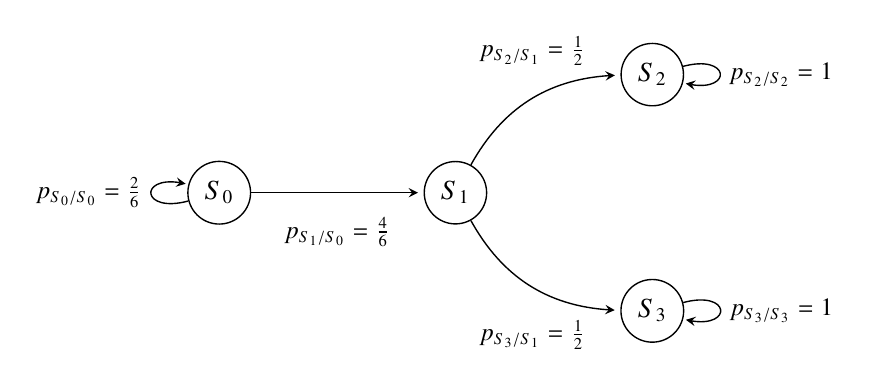
\begin{tikzpicture}[->, >= stealth, shorten >=2pt, line width=0.5pt, node distance=2cm]
  \node[circle, draw] (A) at (0, 1.5) {$S_0$};
  \node[circle, draw] (B) at (3, 1.5) {$S_1$};
  \node[circle, draw] (C) at (5.5, 3) {$S_2$};
  \node[circle, draw] (D) at (5.5, 0) {$S_3$};
  
  \begin{small}
    \path (A) edge [loop left] node [left] {$p_{S_0/S_0} = \frac{2}{6}$} (A);
    \path (A) edge node [below = 0.2cm] {$p_{S_1/S_0} = \frac{4}{6}$} (B);
  
    \path (B) edge [bend left] node [above = 0.3cm] {$p_{S_2/S_1} = \frac{1}{2}$} (C);
    \path (B) edge [bend right] node [below = 0.3cm] {$p_{S_3/S_1} = \frac{1}{2}$} (D);
  
    \path (C) edge [loop right] node {$p_{S_2/S_2} = 1$} (C);
    \path (D) edge [loop right] node {$p_{S_3/S_3} = 1$} (D);
  \end{small}
\end{tikzpicture}
}
    \caption{State diagram generated using LatexTikZ}
    \label{fig:Statediagramdiecoin}
\end{figure}
\end{document}

\section{Altitude}
\documentclass[journal,12pt,two column]{IEEEtran}
%\usepackage{setspace}
\usepackage{amssymb}
\usepackage[cmex10]{amsmath}
\usepackage{amsthm}
\usepackage[export]{adjustbox}
\usepackage{bm}
\def\inputGnumericTable{} 

\usepackage[latin1]{inputenc}                                 
\usepackage{color}                                            
\usepackage{array} 
\usepackage{longtable} 
\usepackage{calc}                                             
\usepackage{multirow}                                         
\usepackage{hhline}                                           
\usepackage{ifthen}  
\usepackage{mathtools}
\usepackage{tikz}
\usepackage{listings}
\usepackage{color}                                            %%
\usepackage{array}                                            %%
\usepackage{caption} 
\usepackage{graphicx}
\renewcommand\thesection{\arabic{section}}
\renewcommand\thesubsection{\thesection.\arabic{subsection}}
\renewcommand\thesubsubsection{\thesubsection.\arabic{subsubsection}}

\renewcommand\thesectiondis{\arabic{section}}
\renewcommand\thesubsectiondis{\thesectiondis.\arabic{subsection}}
\renewcommand\thesubsubsectiondis{\thesubsectiondis.\arabic{subsubsection}}
\title{Assignment}
\author{Barath surya M \\ EE22BTECH11014}

% correct bad hyphenation here
\hyphenation{op-tical net-works semi-conduc-tor}
\def\inputGnumericTable{}                                 %%

\lstset{
%language=C,
frame=single, 
breaklines=true,
columns=fullflexible
}
%\lstset{
%language=tex,
%frame=single, 
%breaklines=true
%}


\providecommand{\pr}[1]{\ensuremath{\Pr\left(#1\right)}}
\providecommand{\prt}[2]{\ensuremath{p_{#1}^{\left(#2\right)} }}        % own macro for this question
\providecommand{\qfunc}[1]{\ensuremath{Q\left(#1\right)}}
\providecommand{\sbrak}[1]{\ensuremath{{}\left[#1\right]}}
\providecommand{\lsbrak}[1]{\ensuremath{{}\left[#1\right.}}
\providecommand{\rsbrak}[1]{\ensuremath{{}\left.#1\right]}}
\providecommand{\brak}[1]{\ensuremath{\left(#1\right)}}
\providecommand{\lbrak}[1]{\ensuremath{\left(#1\right.}}
\providecommand{\rbrak}[1]{\ensuremath{\left.#1\right)}}
\providecommand{\cbrak}[1]{\ensuremath{\left\{#1\right\}}}
\providecommand{\lcbrak}[1]{\ensuremath{\left\{#1\right.}}
\providecommand{\rcbrak}[1]{\ensuremath{\left.#1\right\}}}
\newcommand{\sgn}{\mathop{\mathrm{sgn}}}
\providecommand{\abs}[1]{\left\vert#1\right\vert}
\providecommand{\res}[1]{\Res\displaylimits_{#1}} 
\providecommand{\norm}[1]{\left\lVert#1\right\rVert}
%\providecommand{\norm}[1]{\lVert#1\rVert}
\providecommand{\mtx}[1]{\mathbf{#1}}
\providecommand{\mean}[1]{E\left[ #1 \right]}
\providecommand{\cond}[2]{#1\middle|#2}
\providecommand{\fourier}{\overset{\mathcal{F}}{ \rightleftharpoons}}
%\providecommand{\hilbert}{\overset{\mathcal{H}}{ \rightleftharpoons}}
%\providecommand{\system}{\overset{\mathcal{H}}{ \longleftrightarrow}}
 %\newcommand{\solution}[2]{\textbf{Solution:}{#1}}
\newcommand{\solution}{\noindent \textbf{Solution: }}
\newcommand{\cosec}{\,\text{cosec}\,}
\providecommand{\dec}[2]{\ensuremath{\overset{#1}{\underset{#2}{\gtrless}}}}
\newcommand{\myvec}[1]{\ensuremath{\begin{pmatrix}#1\end{pmatrix}}}
\newcommand{\mydet}[1]{\ensuremath{\begin{vmatrix}#1\end{vmatrix}}}
\providecommand{\rank}{\text{rank}}
\providecommand{\pr}[1]{\ensuremath{\Pr\left(#1\right)}}
\providecommand{\qfunc}[1]{\ensuremath{Q\left(#1\right)}}
 \newcommand*{\permcomb}[4][0mu]{{{}^{#3}\mkern#1#2_{#4}}}
\newcommand*{\perm}[1][-3mu]{\permcomb[#1]{P}}
\newcommand*{\comb}[1][-1mu]{\permcomb[#1]{C}}
\providecommand{\qfunc}[1]{\ensuremath{Q\left(#1\right)}}
\providecommand{\gauss}[2]{\mathcal{N}\ensuremath{\left(#1,#2\right)}}
\providecommand{\diff}[2]{\ensuremath{\frac{d{#1}}{d{#2}}}}
\providecommand{\myceil}[1]{\left \lceil #1 \right \rceil }
\newcommand\figref{Fig.~\ref}
\newcommand\tabref{Table~\ref}
\newcommand{\sinc}{\,\text{sinc}\,}
\newcommand{\rect}{\,\text{rect}\,}
%%
% %\newcommand{\solution}[2]{\textbf{Solution:}{#1}}
%\newcommand{\solution}{\noindent \textbf{Solution:

%\newcommand{\cosec}{\,\text{cosec}\,}
%\numberwithin{equation}{section}
%\numberwithin{equation}{subsection}
%\numberwithin{problem}{section}
%\numberwithin{definition}{section}
%\makeatletter
%\@addtoreset{figure}{problem}
%\makeatother

%\let\StandardTheFigure\thefigure
\let\vec\mathbf

\begin{document}
\maketitle
Consider the experiment of throwing a die. If a multiple of 3 comes up, throw the die again. If any other number comes up, toss a coin. Find the conditional probability of the event the coin shows a tail, given that  at least one die shows a 3.\\
\solution
Let, the states $S_0$ and $S_1$ describe the outcomes of dice throws.\\
$S_2$ and $S_3$ describe the outcomes of coin toss.
\begin{align}
    S_0 &= \Sigma{\brak{Y=k}} ;k\in{\brak{3,6}}\\
    S_1 &= \Sigma{\brak{Y=k}} ; k\in{\brak{1,2,4,5}}\\
    S_2 &= \text{Outcome of coin toss is heads}\\
    S_3 &= \text{Outcome of coin toss is tails}
\end{align}
Conditional Probability is that "The coin shows tails" given that "at least one die shows a 3".
Since, a Markov chain does not depend on the past outcomes,
\begin{align}
    P_{\brak{S_3 | S_0}}&=P_r\brak{X_n=S_3|X_1 =S_0}
\end{align}
Transition Probability Matrix is given as,
\begin{align}
    P&=\myvec{\frac{1}{3}&\frac{2}{3}&0&0\\
                0&0&\frac{1}{2}&\frac{1}{2}\\
                0&0&1&0\\
                0&0&0&0
                }
\end{align}
And State vector is ,
\begin{align}
    Q_0=\myvec{1&0&0&0}
\end{align}
Since the chain starts form $S_0$ according to Markov chain.
The long term Probability that system will be in each state is called stationary state, and stationary state probability is given as,
\begin{align}
    A\pi&=\pi
\end{align}
where $\pi$ is steady state probability vector.\\So,after long time,
\begin{align}
    Q_1&=Q_0 P\\
    Q_2&=Q_1 P \\
    \vdots\\
    Q_{n}&=Q_{n-1} P
\end{align}
So substituting the state vectors we get,
\begin{align}
    Q_{n}&=Q_0 P^{n}\\
\end{align}
applying limits to find the stationary probability vector,
\begin{align}
     \lim_{n \to \infty} Q_{n}&=Q_0 P^{n}
\end{align} \label{eq:steady}
By substituting the values of $Q_0$ and $P$ in the above equation, We get the steady state probability vector as,
\begin{align}
    \pi&=\myvec{0&0&\frac{1}{2}&\frac{1}{2}}
\end{align}
So, the probability that "coin shows tails" given that "Die shows at least one 3" is,
\begin{align}
    p_{\brak{3|1}} &= \frac{1}{2}
\end{align}
\begin{figure}[ht!]
    \centering
    \resizebox{.9\linewidth}{!}{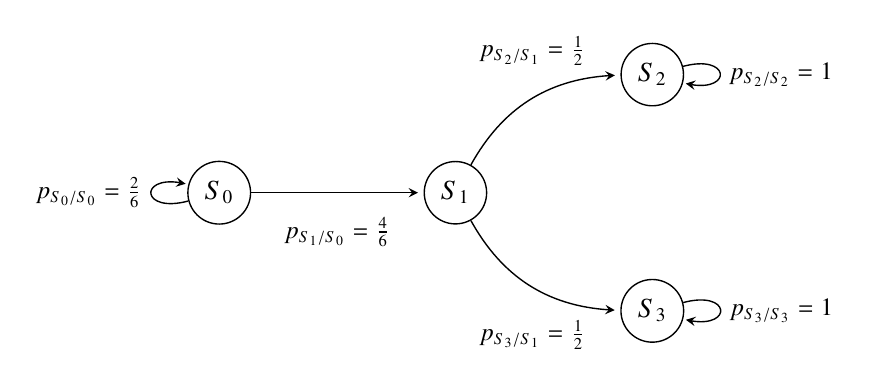
\begin{tikzpicture}[->, >= stealth, shorten >=2pt, line width=0.5pt, node distance=2cm]
  \node[circle, draw] (A) at (0, 1.5) {$S_0$};
  \node[circle, draw] (B) at (3, 1.5) {$S_1$};
  \node[circle, draw] (C) at (5.5, 3) {$S_2$};
  \node[circle, draw] (D) at (5.5, 0) {$S_3$};
  
  \begin{small}
    \path (A) edge [loop left] node [left] {$p_{S_0/S_0} = \frac{2}{6}$} (A);
    \path (A) edge node [below = 0.2cm] {$p_{S_1/S_0} = \frac{4}{6}$} (B);
  
    \path (B) edge [bend left] node [above = 0.3cm] {$p_{S_2/S_1} = \frac{1}{2}$} (C);
    \path (B) edge [bend right] node [below = 0.3cm] {$p_{S_3/S_1} = \frac{1}{2}$} (D);
  
    \path (C) edge [loop right] node {$p_{S_2/S_2} = 1$} (C);
    \path (D) edge [loop right] node {$p_{S_3/S_3} = 1$} (D);
  \end{small}
\end{tikzpicture}
}
    \caption{State diagram generated using LatexTikZ}
    \label{fig:Statediagramdiecoin}
\end{figure}
\end{document}

\section{Perpendicular Bisector}
\documentclass[journal,12pt,two column]{IEEEtran}
%\usepackage{setspace}
\usepackage{amssymb}
\usepackage[cmex10]{amsmath}
\usepackage{amsthm}
\usepackage[export]{adjustbox}
\usepackage{bm}
\def\inputGnumericTable{} 

\usepackage[latin1]{inputenc}                                 
\usepackage{color}                                            
\usepackage{array} 
\usepackage{longtable} 
\usepackage{calc}                                             
\usepackage{multirow}                                         
\usepackage{hhline}                                           
\usepackage{ifthen}  
\usepackage{mathtools}
\usepackage{tikz}
\usepackage{listings}
\usepackage{color}                                            %%
\usepackage{array}                                            %%
\usepackage{caption} 
\usepackage{graphicx}
\renewcommand\thesection{\arabic{section}}
\renewcommand\thesubsection{\thesection.\arabic{subsection}}
\renewcommand\thesubsubsection{\thesubsection.\arabic{subsubsection}}

\renewcommand\thesectiondis{\arabic{section}}
\renewcommand\thesubsectiondis{\thesectiondis.\arabic{subsection}}
\renewcommand\thesubsubsectiondis{\thesubsectiondis.\arabic{subsubsection}}
\title{Assignment}
\author{Barath surya M \\ EE22BTECH11014}

% correct bad hyphenation here
\hyphenation{op-tical net-works semi-conduc-tor}
\def\inputGnumericTable{}                                 %%

\lstset{
%language=C,
frame=single, 
breaklines=true,
columns=fullflexible
}
%\lstset{
%language=tex,
%frame=single, 
%breaklines=true
%}


\providecommand{\pr}[1]{\ensuremath{\Pr\left(#1\right)}}
\providecommand{\prt}[2]{\ensuremath{p_{#1}^{\left(#2\right)} }}        % own macro for this question
\providecommand{\qfunc}[1]{\ensuremath{Q\left(#1\right)}}
\providecommand{\sbrak}[1]{\ensuremath{{}\left[#1\right]}}
\providecommand{\lsbrak}[1]{\ensuremath{{}\left[#1\right.}}
\providecommand{\rsbrak}[1]{\ensuremath{{}\left.#1\right]}}
\providecommand{\brak}[1]{\ensuremath{\left(#1\right)}}
\providecommand{\lbrak}[1]{\ensuremath{\left(#1\right.}}
\providecommand{\rbrak}[1]{\ensuremath{\left.#1\right)}}
\providecommand{\cbrak}[1]{\ensuremath{\left\{#1\right\}}}
\providecommand{\lcbrak}[1]{\ensuremath{\left\{#1\right.}}
\providecommand{\rcbrak}[1]{\ensuremath{\left.#1\right\}}}
\newcommand{\sgn}{\mathop{\mathrm{sgn}}}
\providecommand{\abs}[1]{\left\vert#1\right\vert}
\providecommand{\res}[1]{\Res\displaylimits_{#1}} 
\providecommand{\norm}[1]{\left\lVert#1\right\rVert}
%\providecommand{\norm}[1]{\lVert#1\rVert}
\providecommand{\mtx}[1]{\mathbf{#1}}
\providecommand{\mean}[1]{E\left[ #1 \right]}
\providecommand{\cond}[2]{#1\middle|#2}
\providecommand{\fourier}{\overset{\mathcal{F}}{ \rightleftharpoons}}
%\providecommand{\hilbert}{\overset{\mathcal{H}}{ \rightleftharpoons}}
%\providecommand{\system}{\overset{\mathcal{H}}{ \longleftrightarrow}}
 %\newcommand{\solution}[2]{\textbf{Solution:}{#1}}
\newcommand{\solution}{\noindent \textbf{Solution: }}
\newcommand{\cosec}{\,\text{cosec}\,}
\providecommand{\dec}[2]{\ensuremath{\overset{#1}{\underset{#2}{\gtrless}}}}
\newcommand{\myvec}[1]{\ensuremath{\begin{pmatrix}#1\end{pmatrix}}}
\newcommand{\mydet}[1]{\ensuremath{\begin{vmatrix}#1\end{vmatrix}}}
\providecommand{\rank}{\text{rank}}
\providecommand{\pr}[1]{\ensuremath{\Pr\left(#1\right)}}
\providecommand{\qfunc}[1]{\ensuremath{Q\left(#1\right)}}
 \newcommand*{\permcomb}[4][0mu]{{{}^{#3}\mkern#1#2_{#4}}}
\newcommand*{\perm}[1][-3mu]{\permcomb[#1]{P}}
\newcommand*{\comb}[1][-1mu]{\permcomb[#1]{C}}
\providecommand{\qfunc}[1]{\ensuremath{Q\left(#1\right)}}
\providecommand{\gauss}[2]{\mathcal{N}\ensuremath{\left(#1,#2\right)}}
\providecommand{\diff}[2]{\ensuremath{\frac{d{#1}}{d{#2}}}}
\providecommand{\myceil}[1]{\left \lceil #1 \right \rceil }
\newcommand\figref{Fig.~\ref}
\newcommand\tabref{Table~\ref}
\newcommand{\sinc}{\,\text{sinc}\,}
\newcommand{\rect}{\,\text{rect}\,}
%%
% %\newcommand{\solution}[2]{\textbf{Solution:}{#1}}
%\newcommand{\solution}{\noindent \textbf{Solution:

%\newcommand{\cosec}{\,\text{cosec}\,}
%\numberwithin{equation}{section}
%\numberwithin{equation}{subsection}
%\numberwithin{problem}{section}
%\numberwithin{definition}{section}
%\makeatletter
%\@addtoreset{figure}{problem}
%\makeatother

%\let\StandardTheFigure\thefigure
\let\vec\mathbf

\begin{document}
\maketitle
Consider the experiment of throwing a die. If a multiple of 3 comes up, throw the die again. If any other number comes up, toss a coin. Find the conditional probability of the event the coin shows a tail, given that  at least one die shows a 3.\\
\solution
Let, the states $S_0$ and $S_1$ describe the outcomes of dice throws.\\
$S_2$ and $S_3$ describe the outcomes of coin toss.
\begin{align}
    S_0 &= \Sigma{\brak{Y=k}} ;k\in{\brak{3,6}}\\
    S_1 &= \Sigma{\brak{Y=k}} ; k\in{\brak{1,2,4,5}}\\
    S_2 &= \text{Outcome of coin toss is heads}\\
    S_3 &= \text{Outcome of coin toss is tails}
\end{align}
Conditional Probability is that "The coin shows tails" given that "at least one die shows a 3".
Since, a Markov chain does not depend on the past outcomes,
\begin{align}
    P_{\brak{S_3 | S_0}}&=P_r\brak{X_n=S_3|X_1 =S_0}
\end{align}
Transition Probability Matrix is given as,
\begin{align}
    P&=\myvec{\frac{1}{3}&\frac{2}{3}&0&0\\
                0&0&\frac{1}{2}&\frac{1}{2}\\
                0&0&1&0\\
                0&0&0&0
                }
\end{align}
And State vector is ,
\begin{align}
    Q_0=\myvec{1&0&0&0}
\end{align}
Since the chain starts form $S_0$ according to Markov chain.
The long term Probability that system will be in each state is called stationary state, and stationary state probability is given as,
\begin{align}
    A\pi&=\pi
\end{align}
where $\pi$ is steady state probability vector.\\So,after long time,
\begin{align}
    Q_1&=Q_0 P\\
    Q_2&=Q_1 P \\
    \vdots\\
    Q_{n}&=Q_{n-1} P
\end{align}
So substituting the state vectors we get,
\begin{align}
    Q_{n}&=Q_0 P^{n}\\
\end{align}
applying limits to find the stationary probability vector,
\begin{align}
     \lim_{n \to \infty} Q_{n}&=Q_0 P^{n}
\end{align} \label{eq:steady}
By substituting the values of $Q_0$ and $P$ in the above equation, We get the steady state probability vector as,
\begin{align}
    \pi&=\myvec{0&0&\frac{1}{2}&\frac{1}{2}}
\end{align}
So, the probability that "coin shows tails" given that "Die shows at least one 3" is,
\begin{align}
    p_{\brak{3|1}} &= \frac{1}{2}
\end{align}
\begin{figure}[ht!]
    \centering
    \resizebox{.9\linewidth}{!}{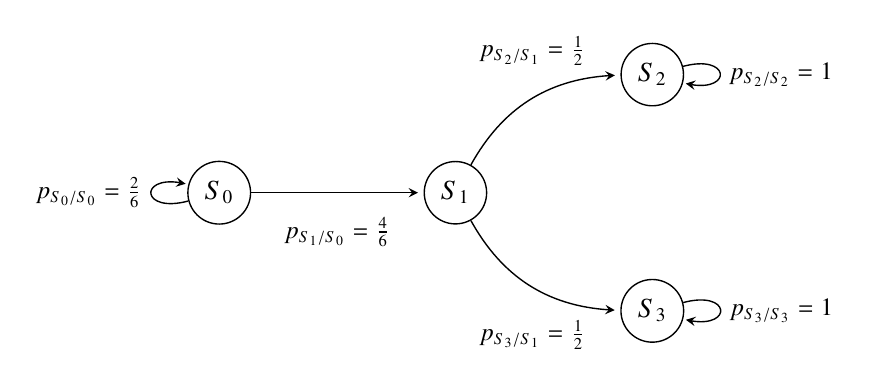
\begin{tikzpicture}[->, >= stealth, shorten >=2pt, line width=0.5pt, node distance=2cm]
  \node[circle, draw] (A) at (0, 1.5) {$S_0$};
  \node[circle, draw] (B) at (3, 1.5) {$S_1$};
  \node[circle, draw] (C) at (5.5, 3) {$S_2$};
  \node[circle, draw] (D) at (5.5, 0) {$S_3$};
  
  \begin{small}
    \path (A) edge [loop left] node [left] {$p_{S_0/S_0} = \frac{2}{6}$} (A);
    \path (A) edge node [below = 0.2cm] {$p_{S_1/S_0} = \frac{4}{6}$} (B);
  
    \path (B) edge [bend left] node [above = 0.3cm] {$p_{S_2/S_1} = \frac{1}{2}$} (C);
    \path (B) edge [bend right] node [below = 0.3cm] {$p_{S_3/S_1} = \frac{1}{2}$} (D);
  
    \path (C) edge [loop right] node {$p_{S_2/S_2} = 1$} (C);
    \path (D) edge [loop right] node {$p_{S_3/S_3} = 1$} (D);
  \end{small}
\end{tikzpicture}
}
    \caption{State diagram generated using LatexTikZ}
    \label{fig:Statediagramdiecoin}
\end{figure}
\end{document}

\section{Angle Bisector}
\documentclass[journal,12pt,two column]{IEEEtran}
%\usepackage{setspace}
\usepackage{amssymb}
\usepackage[cmex10]{amsmath}
\usepackage{amsthm}
\usepackage[export]{adjustbox}
\usepackage{bm}
\def\inputGnumericTable{} 

\usepackage[latin1]{inputenc}                                 
\usepackage{color}                                            
\usepackage{array} 
\usepackage{longtable} 
\usepackage{calc}                                             
\usepackage{multirow}                                         
\usepackage{hhline}                                           
\usepackage{ifthen}  
\usepackage{mathtools}
\usepackage{tikz}
\usepackage{listings}
\usepackage{color}                                            %%
\usepackage{array}                                            %%
\usepackage{caption} 
\usepackage{graphicx}
\renewcommand\thesection{\arabic{section}}
\renewcommand\thesubsection{\thesection.\arabic{subsection}}
\renewcommand\thesubsubsection{\thesubsection.\arabic{subsubsection}}

\renewcommand\thesectiondis{\arabic{section}}
\renewcommand\thesubsectiondis{\thesectiondis.\arabic{subsection}}
\renewcommand\thesubsubsectiondis{\thesubsectiondis.\arabic{subsubsection}}
\title{Assignment}
\author{Barath surya M \\ EE22BTECH11014}

% correct bad hyphenation here
\hyphenation{op-tical net-works semi-conduc-tor}
\def\inputGnumericTable{}                                 %%

\lstset{
%language=C,
frame=single, 
breaklines=true,
columns=fullflexible
}
%\lstset{
%language=tex,
%frame=single, 
%breaklines=true
%}


\providecommand{\pr}[1]{\ensuremath{\Pr\left(#1\right)}}
\providecommand{\prt}[2]{\ensuremath{p_{#1}^{\left(#2\right)} }}        % own macro for this question
\providecommand{\qfunc}[1]{\ensuremath{Q\left(#1\right)}}
\providecommand{\sbrak}[1]{\ensuremath{{}\left[#1\right]}}
\providecommand{\lsbrak}[1]{\ensuremath{{}\left[#1\right.}}
\providecommand{\rsbrak}[1]{\ensuremath{{}\left.#1\right]}}
\providecommand{\brak}[1]{\ensuremath{\left(#1\right)}}
\providecommand{\lbrak}[1]{\ensuremath{\left(#1\right.}}
\providecommand{\rbrak}[1]{\ensuremath{\left.#1\right)}}
\providecommand{\cbrak}[1]{\ensuremath{\left\{#1\right\}}}
\providecommand{\lcbrak}[1]{\ensuremath{\left\{#1\right.}}
\providecommand{\rcbrak}[1]{\ensuremath{\left.#1\right\}}}
\newcommand{\sgn}{\mathop{\mathrm{sgn}}}
\providecommand{\abs}[1]{\left\vert#1\right\vert}
\providecommand{\res}[1]{\Res\displaylimits_{#1}} 
\providecommand{\norm}[1]{\left\lVert#1\right\rVert}
%\providecommand{\norm}[1]{\lVert#1\rVert}
\providecommand{\mtx}[1]{\mathbf{#1}}
\providecommand{\mean}[1]{E\left[ #1 \right]}
\providecommand{\cond}[2]{#1\middle|#2}
\providecommand{\fourier}{\overset{\mathcal{F}}{ \rightleftharpoons}}
%\providecommand{\hilbert}{\overset{\mathcal{H}}{ \rightleftharpoons}}
%\providecommand{\system}{\overset{\mathcal{H}}{ \longleftrightarrow}}
 %\newcommand{\solution}[2]{\textbf{Solution:}{#1}}
\newcommand{\solution}{\noindent \textbf{Solution: }}
\newcommand{\cosec}{\,\text{cosec}\,}
\providecommand{\dec}[2]{\ensuremath{\overset{#1}{\underset{#2}{\gtrless}}}}
\newcommand{\myvec}[1]{\ensuremath{\begin{pmatrix}#1\end{pmatrix}}}
\newcommand{\mydet}[1]{\ensuremath{\begin{vmatrix}#1\end{vmatrix}}}
\providecommand{\rank}{\text{rank}}
\providecommand{\pr}[1]{\ensuremath{\Pr\left(#1\right)}}
\providecommand{\qfunc}[1]{\ensuremath{Q\left(#1\right)}}
 \newcommand*{\permcomb}[4][0mu]{{{}^{#3}\mkern#1#2_{#4}}}
\newcommand*{\perm}[1][-3mu]{\permcomb[#1]{P}}
\newcommand*{\comb}[1][-1mu]{\permcomb[#1]{C}}
\providecommand{\qfunc}[1]{\ensuremath{Q\left(#1\right)}}
\providecommand{\gauss}[2]{\mathcal{N}\ensuremath{\left(#1,#2\right)}}
\providecommand{\diff}[2]{\ensuremath{\frac{d{#1}}{d{#2}}}}
\providecommand{\myceil}[1]{\left \lceil #1 \right \rceil }
\newcommand\figref{Fig.~\ref}
\newcommand\tabref{Table~\ref}
\newcommand{\sinc}{\,\text{sinc}\,}
\newcommand{\rect}{\,\text{rect}\,}
%%
% %\newcommand{\solution}[2]{\textbf{Solution:}{#1}}
%\newcommand{\solution}{\noindent \textbf{Solution:

%\newcommand{\cosec}{\,\text{cosec}\,}
%\numberwithin{equation}{section}
%\numberwithin{equation}{subsection}
%\numberwithin{problem}{section}
%\numberwithin{definition}{section}
%\makeatletter
%\@addtoreset{figure}{problem}
%\makeatother

%\let\StandardTheFigure\thefigure
\let\vec\mathbf

\begin{document}
\maketitle
Consider the experiment of throwing a die. If a multiple of 3 comes up, throw the die again. If any other number comes up, toss a coin. Find the conditional probability of the event the coin shows a tail, given that  at least one die shows a 3.\\
\solution
Let, the states $S_0$ and $S_1$ describe the outcomes of dice throws.\\
$S_2$ and $S_3$ describe the outcomes of coin toss.
\begin{align}
    S_0 &= \Sigma{\brak{Y=k}} ;k\in{\brak{3,6}}\\
    S_1 &= \Sigma{\brak{Y=k}} ; k\in{\brak{1,2,4,5}}\\
    S_2 &= \text{Outcome of coin toss is heads}\\
    S_3 &= \text{Outcome of coin toss is tails}
\end{align}
Conditional Probability is that "The coin shows tails" given that "at least one die shows a 3".
Since, a Markov chain does not depend on the past outcomes,
\begin{align}
    P_{\brak{S_3 | S_0}}&=P_r\brak{X_n=S_3|X_1 =S_0}
\end{align}
Transition Probability Matrix is given as,
\begin{align}
    P&=\myvec{\frac{1}{3}&\frac{2}{3}&0&0\\
                0&0&\frac{1}{2}&\frac{1}{2}\\
                0&0&1&0\\
                0&0&0&0
                }
\end{align}
And State vector is ,
\begin{align}
    Q_0=\myvec{1&0&0&0}
\end{align}
Since the chain starts form $S_0$ according to Markov chain.
The long term Probability that system will be in each state is called stationary state, and stationary state probability is given as,
\begin{align}
    A\pi&=\pi
\end{align}
where $\pi$ is steady state probability vector.\\So,after long time,
\begin{align}
    Q_1&=Q_0 P\\
    Q_2&=Q_1 P \\
    \vdots\\
    Q_{n}&=Q_{n-1} P
\end{align}
So substituting the state vectors we get,
\begin{align}
    Q_{n}&=Q_0 P^{n}\\
\end{align}
applying limits to find the stationary probability vector,
\begin{align}
     \lim_{n \to \infty} Q_{n}&=Q_0 P^{n}
\end{align} \label{eq:steady}
By substituting the values of $Q_0$ and $P$ in the above equation, We get the steady state probability vector as,
\begin{align}
    \pi&=\myvec{0&0&\frac{1}{2}&\frac{1}{2}}
\end{align}
So, the probability that "coin shows tails" given that "Die shows at least one 3" is,
\begin{align}
    p_{\brak{3|1}} &= \frac{1}{2}
\end{align}
\begin{figure}[ht!]
    \centering
    \resizebox{.9\linewidth}{!}{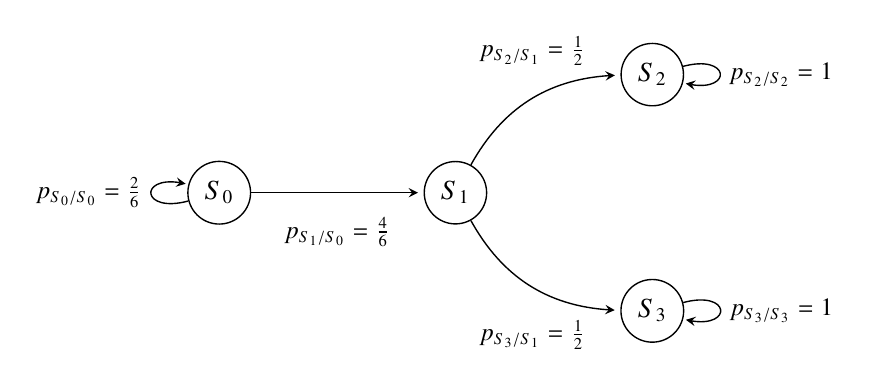
\begin{tikzpicture}[->, >= stealth, shorten >=2pt, line width=0.5pt, node distance=2cm]
  \node[circle, draw] (A) at (0, 1.5) {$S_0$};
  \node[circle, draw] (B) at (3, 1.5) {$S_1$};
  \node[circle, draw] (C) at (5.5, 3) {$S_2$};
  \node[circle, draw] (D) at (5.5, 0) {$S_3$};
  
  \begin{small}
    \path (A) edge [loop left] node [left] {$p_{S_0/S_0} = \frac{2}{6}$} (A);
    \path (A) edge node [below = 0.2cm] {$p_{S_1/S_0} = \frac{4}{6}$} (B);
  
    \path (B) edge [bend left] node [above = 0.3cm] {$p_{S_2/S_1} = \frac{1}{2}$} (C);
    \path (B) edge [bend right] node [below = 0.3cm] {$p_{S_3/S_1} = \frac{1}{2}$} (D);
  
    \path (C) edge [loop right] node {$p_{S_2/S_2} = 1$} (C);
    \path (D) edge [loop right] node {$p_{S_3/S_3} = 1$} (D);
  \end{small}
\end{tikzpicture}
}
    \caption{State diagram generated using LatexTikZ}
    \label{fig:Statediagramdiecoin}
\end{figure}
\end{document}


\end{document}

 
